\chapter{保证项目质量}
关键词:产生软件质量问题的13个原因
\section{项目质量管理概述}
\subsection{质量和质量管理}
\subsubsection{质量的定义}
A. 国际标准化组织 ( ISO ) 对质量的定义:
\par 质量是反映实体满足明确和隐含需要的能力的特性总和。
\par B. 质量定义
\par 质量是通过实体来体现的,质量的实体可以是产品,也可以是某项活动或过程的工作质量,还可以是质量管理体系运行的质量。
\par 质量的内涵:
\begin{itemize}
	\item 内在质量特性:性能、特性、强度、精度。
	\item 外在质量特性:外形、包装、装潢、色泽、味道。
	\item 经济质量特性:寿命、成本、价格、运营维护费用。
	\item 商业质量特性:保持期、保修期、售后服务水平。
	\item 环保质量特性:产品对于环境保护或环境污染。
\end{itemize}
\par 软件质量的质量特性:
\begin{itemize}
	\item 功能性:适合性、准确性、互操作性、依从性、安全性;
	\item 可靠性:成熟性、容错性、易恢复性;
	\item 易用性:易理解性、易学性、易操作性;
	\item 效率:时间特性、资源特性;
	\item 可维护性:易分析性、易改变性、稳定性、易测试性;
	\item 可移植性:适应性、易安装性、遵循性、易替换性。
\end{itemize}
\subsection{质量和质量管理}
ISO将质量管理定义为:“\textbf{在质量方面指挥和控制组织的协调活动。} ”
\par 质量管理是确定质量方针、目标和职责,并在质量体系中通过诸如质量策划、质量控制、质量保障和质量改进使质量得以实现的全部管理活动。
\par 注:
\begin{enumerate}
	\item 质量管理作为企业管理活动,贯穿企业从质量方针制定到用户对项目产品质量的最终检验的\textbf{全过程};
	\item 质量管理需要\textbf{所有项目干系人}的共同努力;
	\item 质量管理不仅仅是\textbf{产品的质量}管理,而且还包括制造产品过程中\textbf{工作质量}的管理。
\end{enumerate}
\subsubsection{IT项目质量管理}
项目的质量管理:指围绕项目质量所进行的指挥、协调和控制等活动。
\par IT项目质量管理:指IT企业为了使其产品和服务质量能满足不断更新的市场与客户的质量要求而开展的策划、组织、计划、实施、控制、改进活动的总和。
\par 需要注意的是:
\begin{itemize}
	\item 质量是软件企业的生命线,质量管理是全体员工的责任;
	\item 使顾客满意是质量管理的目的;
	\item 质量不是检测出来的,而是策划和制造出来的;
	\item 建立项目管理规范、标准和模板是项目质量的基本保障;
	\item 质量管理的关键是不断地改进和提高项目管理能力;
	\item 管理者对产品的质量负责。
\end{itemize}
\subsection{质量管理过程}
\begin{enumerate}
	\item 质量规划:确定适合于项目的质量标准并决定如何满足这些标准。
	\item 质量保证:开展有计划、有系统的质量活动,确保项目的所有过程满足干系人的期望。
	\item 质量控制:监控具体项目过程与结果,以确定其是否符合相关质量标准。制定有效方案,以消除产生质量问题的原因。
\end{enumerate}
\begin{figure}[!h]
	\centering
	
\includegraphics[width=0.8\textwidth]{image/7-1}
	\caption{质量管理过程}
\end{figure}
\subsection{现代质量管理}
质量管理的发展,按照所依据的手段和方式来划分,大致经过三个阶段
\begin{itemize}
	\item 质量检验阶段:通过严格检验来控制和保证产品质量,对质量管理的理解还只限于质量的检验;
	\item 统计质量控制阶段:利用数理统计原理在生产工序间进行质量控制,预防产生不合格品并检验产品的质量;
	\item 全面质量管理阶段:从过去的事后检验和把关为主转变为预防和改进为主;从管结果变为管因素,发动全员、全部门参加,使生产的全过程都处于受控状态。
\end{itemize}
\section{质量管理体系与方法}
质量管理体系是指在质量方面指挥和控制组织的管理体系,由建立质量方针和目标并实现这些目标的相互关联或相互作用的一组要素组成。
\subsection{戴明改进循环}
质量管理工作过程总结为PDCA四个阶段:计划、执行、检查、改进。
\begin{figure}[!h]
	\centering
	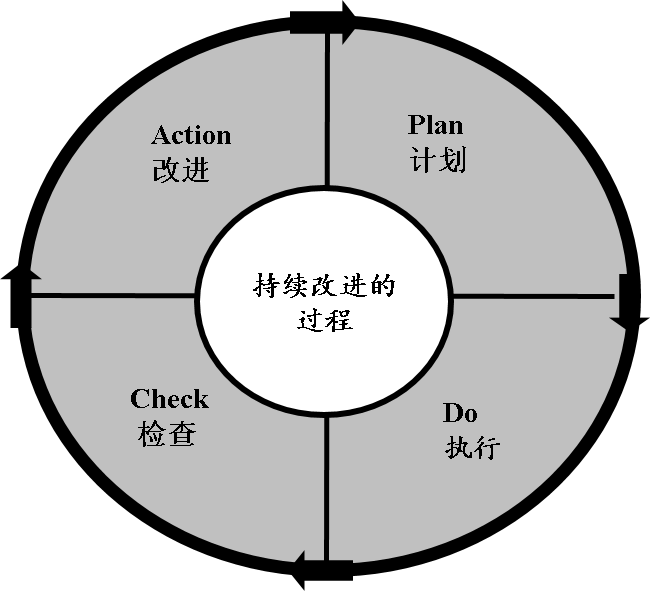
\includegraphics[width=0.3\textwidth]{image/7-2}
	\caption{戴明改进循环}
\end{figure}
\subsection{ISO9000质量认证体系}
质量认证按认证的对象分为产品质量认证和质量体系认证两类;按认证的作用可分为安全认证和合格认证。
\par ISO9000 是涉及质量保证与质量管理活动的一簇标准的统称。它提供了一个组织满足其质量认证标准的最低要求,健全了质量保证体系认证制度。
\par  ISO9000 的8项质量管理原则:以顾客为中心、领导作用、全员参与、过程方法、管理的系统方法、持续改进、基于事实的决策方法、互利的供方关系。
\subsection{软件能力成熟度模型}
成熟度模型:用于帮助组织改进过程和系统的框架模型。
\par 目前在软件行业应用最为广泛的软件生产工程标准是软件能力成熟度模型(CMM)。
\par CMM分为5个等级:
\begin{enumerate}
	\item 初始级。表明软件项目开发过程无序,进度、预算、功能和质量等方面不可预测;
	\item 可重复级。企业过程已制度化,有纪律,可重复;
	\item 已定义级。企业过程已实现标准化;
	\item 已管理级,企业已实现过程的定量化;
	\item 优化级,企业过程可自发地不断改进,能够防止同类问题二次出现。
\end{enumerate}
\par \textbf{软件质量保证}的目标:
\begin{enumerate}
	\item 对软件质量保证活动做到有计划;
	\item 客观地验证软件产品及其活动是否遵守应用的标准、规程和需求;
	\item 将软件质量保证活动及其结果及时通知相关小组和个人;
	\item 由上级管理部门及时处理软件项目内部解决不了的不一致性问题。
\end{enumerate}
\par \textbf{软件质量管理}的目标:
\begin{enumerate}
	\item 项目的软件质量管理活动是有计划的;
	\item 软件产品质量的可测目标和目标的优先级被定义;
	\item 实现软件产品质量的实际进展过程被量化。
\end{enumerate}
\subsection{软件质量改进的问题与对策}
\begin{itemize}
	\item 要重视效果,不要徒有虚名。
	\item 要循序渐进,不要急于求成。
	\item 要注重实际,不要照抄照搬。
	\item 要把握重点,不要遍地开花。
	\item 要注重过程,不要只重结果。
	\item 要争取客户支持,不要一味“埋头苦干”
\end{itemize}
\section{项目质量规划}
质量规划是实施规划过程组和制定项目计划期间的若干关键过程之一,因此应与其他项目规划过程结合进行。
\par 质量规划的任务:识别哪些质量标准适应本项目,并确定如何满足这些标准的要求。
\par 注:质量在计划中确定,而非在检验中确定。
\par 编制质量计划主要考虑:
\begin{enumerate}
	\item 明确质量标准:确定每个独特项目的相关质量标准,把质量规划到项目的产品和管理项目所涉及的过程之中。
	\item 确定关键因素:理解哪个变量影响结果是质量计划编制的重要部分。 
	\item 建立控制流程:以一种能理解的、完整的形式传达为确保质量而采取的纠正措施。
\end{enumerate}
\subsection{质量规划依据}
事业环境因素、组织过程资产 、项目范围说明书、项目产品说明书、项目管理计划。
\subsection{质量规划工具与技术}
成本效益分析法 、质量标杆法 、流程图法 、实验设计法、其他质量规划工具 。
\subsection{质量规划成果}
质量管理计划、质量测试指标、质量核对表、可用于其它管理的信息 。
\section{项目质量保证}
质量保证指通过实施计划中的系统质量活动,确保项目实施满足要求所需的所有过程。
\par 质量保证的作用是从外部向质量控制系统施加影响与压力,促使质量管理活动更有效进行。
\subsection{质量保证的意义}
\begin{enumerate}
	\item 为了提供信用,证明项目将会达到有关质量标准,而在质量体系中开展的有计划、有组织的工作活动。
	\item 可以向项目管理小组和执行组织提供(内部质量保证),或者向客户和其他没有介入项目工作的人员提供(外部质量保证)。
\end{enumerate}
\subsection{项目质量保证过程}
项目质量保证的依据:质量规划过程获得的项目质量管理计划、质量测试指标、过程改进计划,以及在其他过程中获得的批准的变更请求、质量控制测量、实施的变更请求、实施的纠正措施、实施的预防措施、实施的缺陷补救和工作绩效信息等。
\par 质量保证的成果:
\begin{enumerate}
	\item 请求的变更,以提高组织的质量政策、过程和程序的效率和效益;
	\item 在进行质量保证活动后采取地纠正措施;
	\item 以及更新的组织过程资产和更新的项目管理计划。
\end{enumerate}
\subsection{软件质量保证}
软件质量保证(SQA)是为了使软件开发的流程按照事先定义的规范进行,以保证软件质量活动。
\par SQA的工作流程与步骤:
\begin{enumerate}
	\item 建立SQA小组;
	\item 选择和确定SQA小组活动,并作为SQA计划的重要输入;
	\item 制定SQA计划,明确SQA活动与整个软件开发生命周期中各个阶段的关系;
	\item 执行SQA计划、对相关人员进行培训、选择与整个软件工程环境相适应的质量保证工具;
	\item 不断完善质量保证过程活动中存在的不足,改进项目的质量保证过程。
\end{enumerate}
\par 一般把SQA活动分为以下五类:
\begin{itemize}
	\item 评审软件产品、工具与设施
	\item SQA活动审查的软件开发过程
	\item 参与技术和管理评审
	\item 形成SQA报告
	\item 处理相互关系
\end{itemize}
\section{项目质量控制}
质量控制(Quality Control,QC)指采取有效措施监控项目的执行结果,以确定它们是否符合有关的项目质量标准,并确定适当方式消除导致项目绩效令人不满意的原因。
\par 目标:确保项目质量能满足项目干系人提出的适用性、可靠性、安全性等质量要求。
\par 范围:项目质量形成全过程的各个环节。
\subsection{实施质量控制}
项目的质量控制主要从以下两个方面进行:
\begin{itemize}
	\item 项目产品或服务的质量控制
	\item 项目管理过程的质量控制
\end{itemize}
\subsection{质量控制工具与技术}
因果图、控制图、流程图、直方图、帕累托图、趋势图、散点图等7种工具和技术。
\par 控制图和七点运行法则:如果有连续的7个或7个以上的圆点分布在中心线的同一侧,或者出现同向变化的趋势,即使它们都处于控制界限内,但也意味着其出现了一定的问题或者受到了外界因素的干扰,应将视其为失控状态。 
\subsection{质量控制成果}
质量控制衡量、确认的缺陷补救、更新的质量基准、推荐的纠正措施、推荐的预防措施、请求的变更、推荐的缺陷补救、更新组织过程资产、确认的可交付成果和更新项目管理计划。